\newpage
\section{Auswertung}     

\subsection{Charakteristik des Zählrohrs}
\begin{table}[H]
    \centering
    \begin{tabular}{S [table-format=3.0] S [table-format=3.0] S [table-format=5.0]S [table-format=5.0]}
        \toprule
        {$U \mathbin{\scalebox{1.5} / }\si{\volt}$}& {$N$} & {$U \mathbin{\scalebox{1.5} / }\si{\volt}$}   & {$N$}\\
        \midrule
        320 & 9672  & 520  & 10255 \\ 
        330 & 9689  & 530  & 10151 \\
        340 & 9580  & 540  & 10351 \\
        350 & 9837  & 550  & 10184 \\
        360 & 9886  & 560  & 10137 \\
        370 & 1004  & 570  & 10186 \\
        380 & 9996  & 580  & 10171 \\
        390 & 9943  & 590  & 10171 \\
        400 & 9995  & 600  & 10253 \\
        410 & 9980  & 610  & 10368 \\
        420 & 9986  & 620  & 10365 \\
        430 & 9960  & 630  & 10224 \\
        440 & 10219 & 640  & 10338 \\
        450 & 10264 & 650  & 10493 \\
        460 & 10174 & 660  & 10467 \\
        470 & 10035 & 670  & 10640 \\
        480 & 10350 & 680  & 10939 \\
        490 & 10290 & 690  & 11159 \\
        500 & 10151 & 700  & 11547 \\
        510 & 10110 & /    &  /    \\
        \bottomrule
    \end{tabular}
\caption{Die Messwerte der Spannung gegen die Anzahl der Impulse pro 60/s.}
\label{tab:Mess_Ch}
\end{table}

\noindent Die Daten werden in ein Diagramm eingezeichnet und mit einem Fehlerbalken versehen. Der Fehler entspricht der Wurzel der Anzahl der Impulse.
Durch das Plateau wird eine Ausgleichsgerade der Form $y = mx + b$ gelegt. Die Werte für die Ausgleichsgerade ergeben sich zu:
\begin{align}
    m&= \num{1.138 \pm 0.24} \nonumber \\
    b&= \num{959 \pm 121}    \nonumber
\end{align}

\begin{figure}[H]
    \centering
    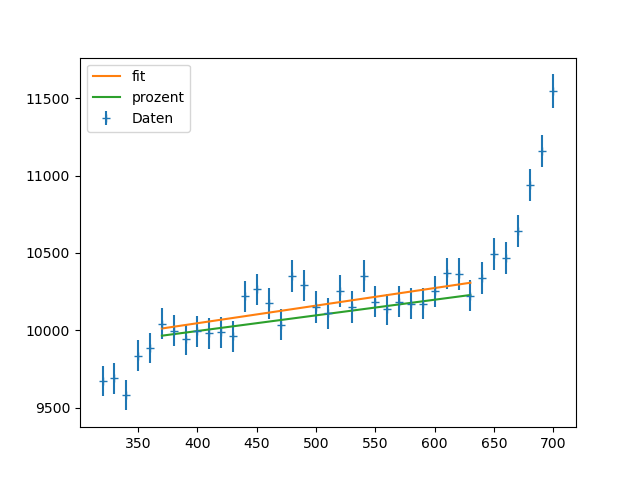
\includegraphics[width=0.85\textwidth]{build/plots/a.png}
    \caption{Die Charasteristik des Zählrohrs mit linearem fit auf dem Plateau.}
    \label{img:plot1}
\end{figure}

\subsection{Totzeit}

\noindent Die Totzeit des Zählrohrs wird näherungsweise mit der Formel:
\begin{equation}
    T \approx \frac{N_1 + N_2 - N_{1+2}}{2N_1N_2}
\end{equation}
\noindent berechnet.Mit folgenden Werten für die Anzahl der Impulse pro 120 Sekunden:

\begin{align} 
    N_1 &= 96041\\
    N_2 &= 76518\\
    N_{1+2} &= 58479\\
\end{align}

\noindent wird die Totzeit $T$ zu $\SI{22.52}{\micro\second}$ berechnet.

\subsection{freigesetzte Ladung}

\noindent Zur Berechnung der Freigesetzten Ladungen pro einfallendem Teilchen werden folgende Werte benutzt:

\begin{table}[H]
    \centering
    \begin{tabular}{S [table-format=3.0] S [table-format=3.0] S [table-format=5.0]S [table-format=5.0]}
        \toprule
        {$U \mathbin{\scalebox{1.5} / }\si{\volt}$} & {$N$} & {$I \mathbin{\scalebox{1.5} / }\si{\micro\ampere}$}\\
        \midrule

        350 & 9837  & 0.3 \\
        400 & 9995  & 0.4 \\
        450 & 10264 & 0.7 \\
        500 & 10151 & 0.8 \\
        550 & 10184 & 1.0 \\
        600 & 10253 & 1.3 \\
        650 & 10493 & 1.4 \\
        700 & 11547 & 1.8 \\
        \bottomrule
    \end{tabular}
\caption{Die Messwerte zur Berechnung der freigesetzten Ladung.}
\label{tab:Mess_q}
\end{table}

\noindent Mittels der Formel:
\begin{equation}
    Z=\frac{I}{e_0N}
\end{equation}
\noindent ergibt sich folgende Graphik:
\begin{figure}[H]
    \centering
    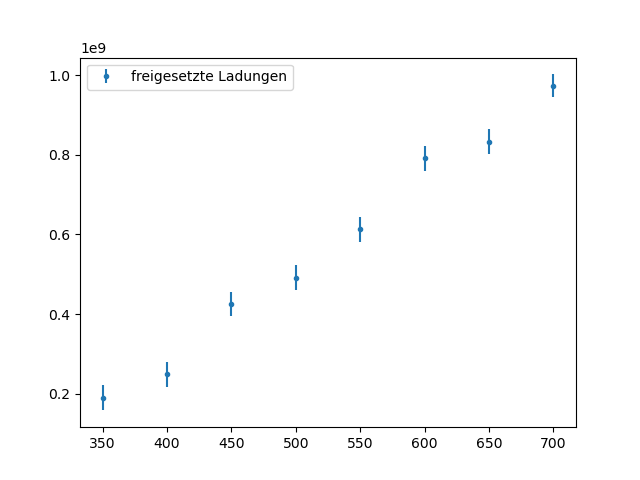
\includegraphics[width=0.85\textwidth]{build/plots/d.png}
    \caption{Ein Plot der freigesetzten Ladungen pro Teilchen gegen die anliegende Spannung.}
    \label{img:plot1}
\end{figure}
\noindent mit den Werten:
\begin{table}[H]
    \centering
    \begin{tabular}{S [table-format=3.0] S [table-format=3.2] @{$\pm{}$} S [table-format=2.2]}
        \toprule
        {$U \mathbin{\scalebox{1.5} / }\si{\volt}$} & {$Z_{\text{Werte}} * 10^6$} & {$Z_{\text{Unsicherheit}} 10^{6}$}\\
        \midrule
        350 & 190.36 & 31.78 \\
        400 & 249.81 & 31.32 \\
        450 & 425.71 & 30.69 \\
        500 & 491.94 & 31.13 \\
        550 & 612.94 & 31.24 \\
        600 & 791.46 & 31.42 \\
        650 & 832.84 & 30.83 \\
        700 & 973.06 & 28.50 \\
        \bottomrule
    \end{tabular}
\caption{Die Messwerte zur Berechnung der freigesetzten Ladung.}
\label{tab:Mess_q}
\end{table}



